% !TEX root =../pfcTipoETSI.tex
\chapter{Ala acuática bidimensional}\LABCHAP{ala2D}
\pagestyle{esitscCD}
\epigraph{ }{}

%\lettrine[lraise=0.7, lines=1, loversize=-0.25]{E}{l} 
\lettrine[lraise=-0.1, lines=2, loversize=0.25]{A}l final del capítulo anterior se expuso la posibilidad de emplear los gradientes favorables de presión se producen en el borde de ataque de un perfil aerodinámico (cuando sobre el incide una corriente con un ángulo de ataque $\alpha$ determinado) como mecanismo para la formación de microburbujas monodispersas, basándose por analogía en los resultados de~\cite{Evangelio2015b}. El objetivo de este capítulo es pues materializar esta idea diseñando, fabricando y realizando experimentos con un dispositivo generador masivo de microburbujas consistente en un perfil aerodinámico\footnote{El diseño de un ala para que pueda realizarse la hipótesis de perfil bidimensional no es trivial, por lo que esta cuestión se abordará con el debido detalle en la \SSEC{DisenoAla}.}. De este modo, se pretende no sólo demostrar que la producción de burbujas de tamaños milimétricos y submilimétricos no lleva necesariamente aparejado el empleo de dispositivos microfluídicos. Además, se contrastarán las hipótesis realizadas en el capítulo anterior y se explorarán las diferentes dificultades que puedan presentarse en el proceso de escalado. 

La estructura que tomará el capítulo será la siguiente: 
\begin{enumerate}
\item En la \SEC{dessign}, se describe todo lo concerniente al diseño y fabricación del modelo completo, que comprende el dispositivo generador de microburbujas y el montaje experimental del mismo. 
\item En la \SEC{experimentos2D}, se especifican los métodos de experimentación y análisis que serán empleados en la obtención de resultados. De este modo, se describirá la configuración final del \textit{set-up}, el protocolo de experimentación, los datos en bruto obtenidos y el posterior tratamiento para el análisis de los mismos.
\item Finalmente, en  la \SEC{results2D}, se muestran y comentan los resultados obtenidos, realizando las conclusiones pertinentes al final del capítulo
\end{enumerate}

\section{Diseño y fabricación}\LABSEC{dessign}

El objetivo de esta sección es describir de forma detallada los parámetros que configuran el diseño del modelo, tanto aquellos que se refieren al dispositivo en sí como al montaje experimental. Para ello, se describen sucintamente en primer lugar los equipos de los que se dispone y las distintas limitaciones de cada uno de ellos, con el fin de poder acotar el diseño final.

\subsection{Equipos disponibles y limitaciones}\LABSSEC{equipos}

La implementación de esta prueba de concepto consistente en un perfil bidimensional implica que la forma más sencilla de crear una corriente relativa entre el fluido y el perfil sea fijando este último y haciendo incidir sobre él un líquido a la velocidad uniforme $U_{\infty}$; esta implementación puede realizarse perfectamente en un túnel hidrodinámico. Por otro lado, se precisará de un sistema de inyección de aire que permita la formación de las burbujas, por lo que se requiere una linea de presión acompañada de manorreductores que permitan abordar esta tarea. Finalmente, para poder obtener y posteriormente analizar los datos extraídos del experimento, será necesario poder documentarlo, para lo cual se hará uso de una cámara de vídeo. Esta cámara no puede ser cualquiera, ya que el fenómeno que se pretende grabar ocurre en unas pocas fracciones de segundo. En efecto, si se pretenden obtener con este dispositivo burbujas de tamaños comparables a las encontradas en~\cite{Evangelio2015b}, esto es $d_{b}\sim \mathcal{O}\left(200\,\mathrm{\mu m}\right)$, y se estima que las burbujas son convectadas aguas abajo del perfil a una velocidad\footnote{En~\cite{Evngelio2015b}, las burbujas son convectadas a la velocidad de la corriente, siendo en este caso $U$ la velocidad media en el capilar para $Re \gg 1$.} $v \sim U_{\infty}$, se tendrá que una burbuja recorre una distancia del orden de su diámetro en un tiempo $t_{b} \sim d_{b}/U_{\infty} \sim \mathcal{O}\left(200\,\mathrm{\mu s}\right)$, por lo que serán necesarios del orden de 5000~fotogramas por segundo (en adelante fps): se necesita, por lo tanto, una cámara de alta velocidad. 

\subsubsection*{Tunel hidrodinámico}

En el laboratorio de Mecánica de Fluidos de la Escuela Superior de Ingeniería de Sevilla se dispone de un túnel hidrodinámico como el mostrado en la \FIG{tunel}. Como puede observarse en la figura, el túnel consiste en un conducto de sección rectangular a través del cual se hace circular un líquido (en este caso agua) utilizando para ello una bomba. Una vez que la bomba ha hecho ascender al líquido hasta la altura adecuada, se le hace pasar a través de una cámara de contracción cuyo fin es uniformizar el flujo incidente en la cámara de ensayos (zona transparente del túnel). Pese a no apreciarse en la imagen, el túnel se encuentra abierto  y en contacto con la atmósfera en su parte superior, mientras que la parte inferior del mismo también esta formada por cristales de igual transparencia que las paredes laterales. Las dimensiones del túnel pueden consultarse en la \TAB{tunel}

\begin{table}
\begin{tabular}{c c}
\textbf{Dimensión} & Valor [cm] \\
\hline \hline
Ancho de la sección & slka  \\
Altura de la secció & sajfios \\
distancia entre soportes & fljisd \\
\hline
\end{tabular}
\caption{Dimensiones relevantes del túnel hidrodinámico}
\LABTAB{tunel}
\end{table}

\begin{figure}
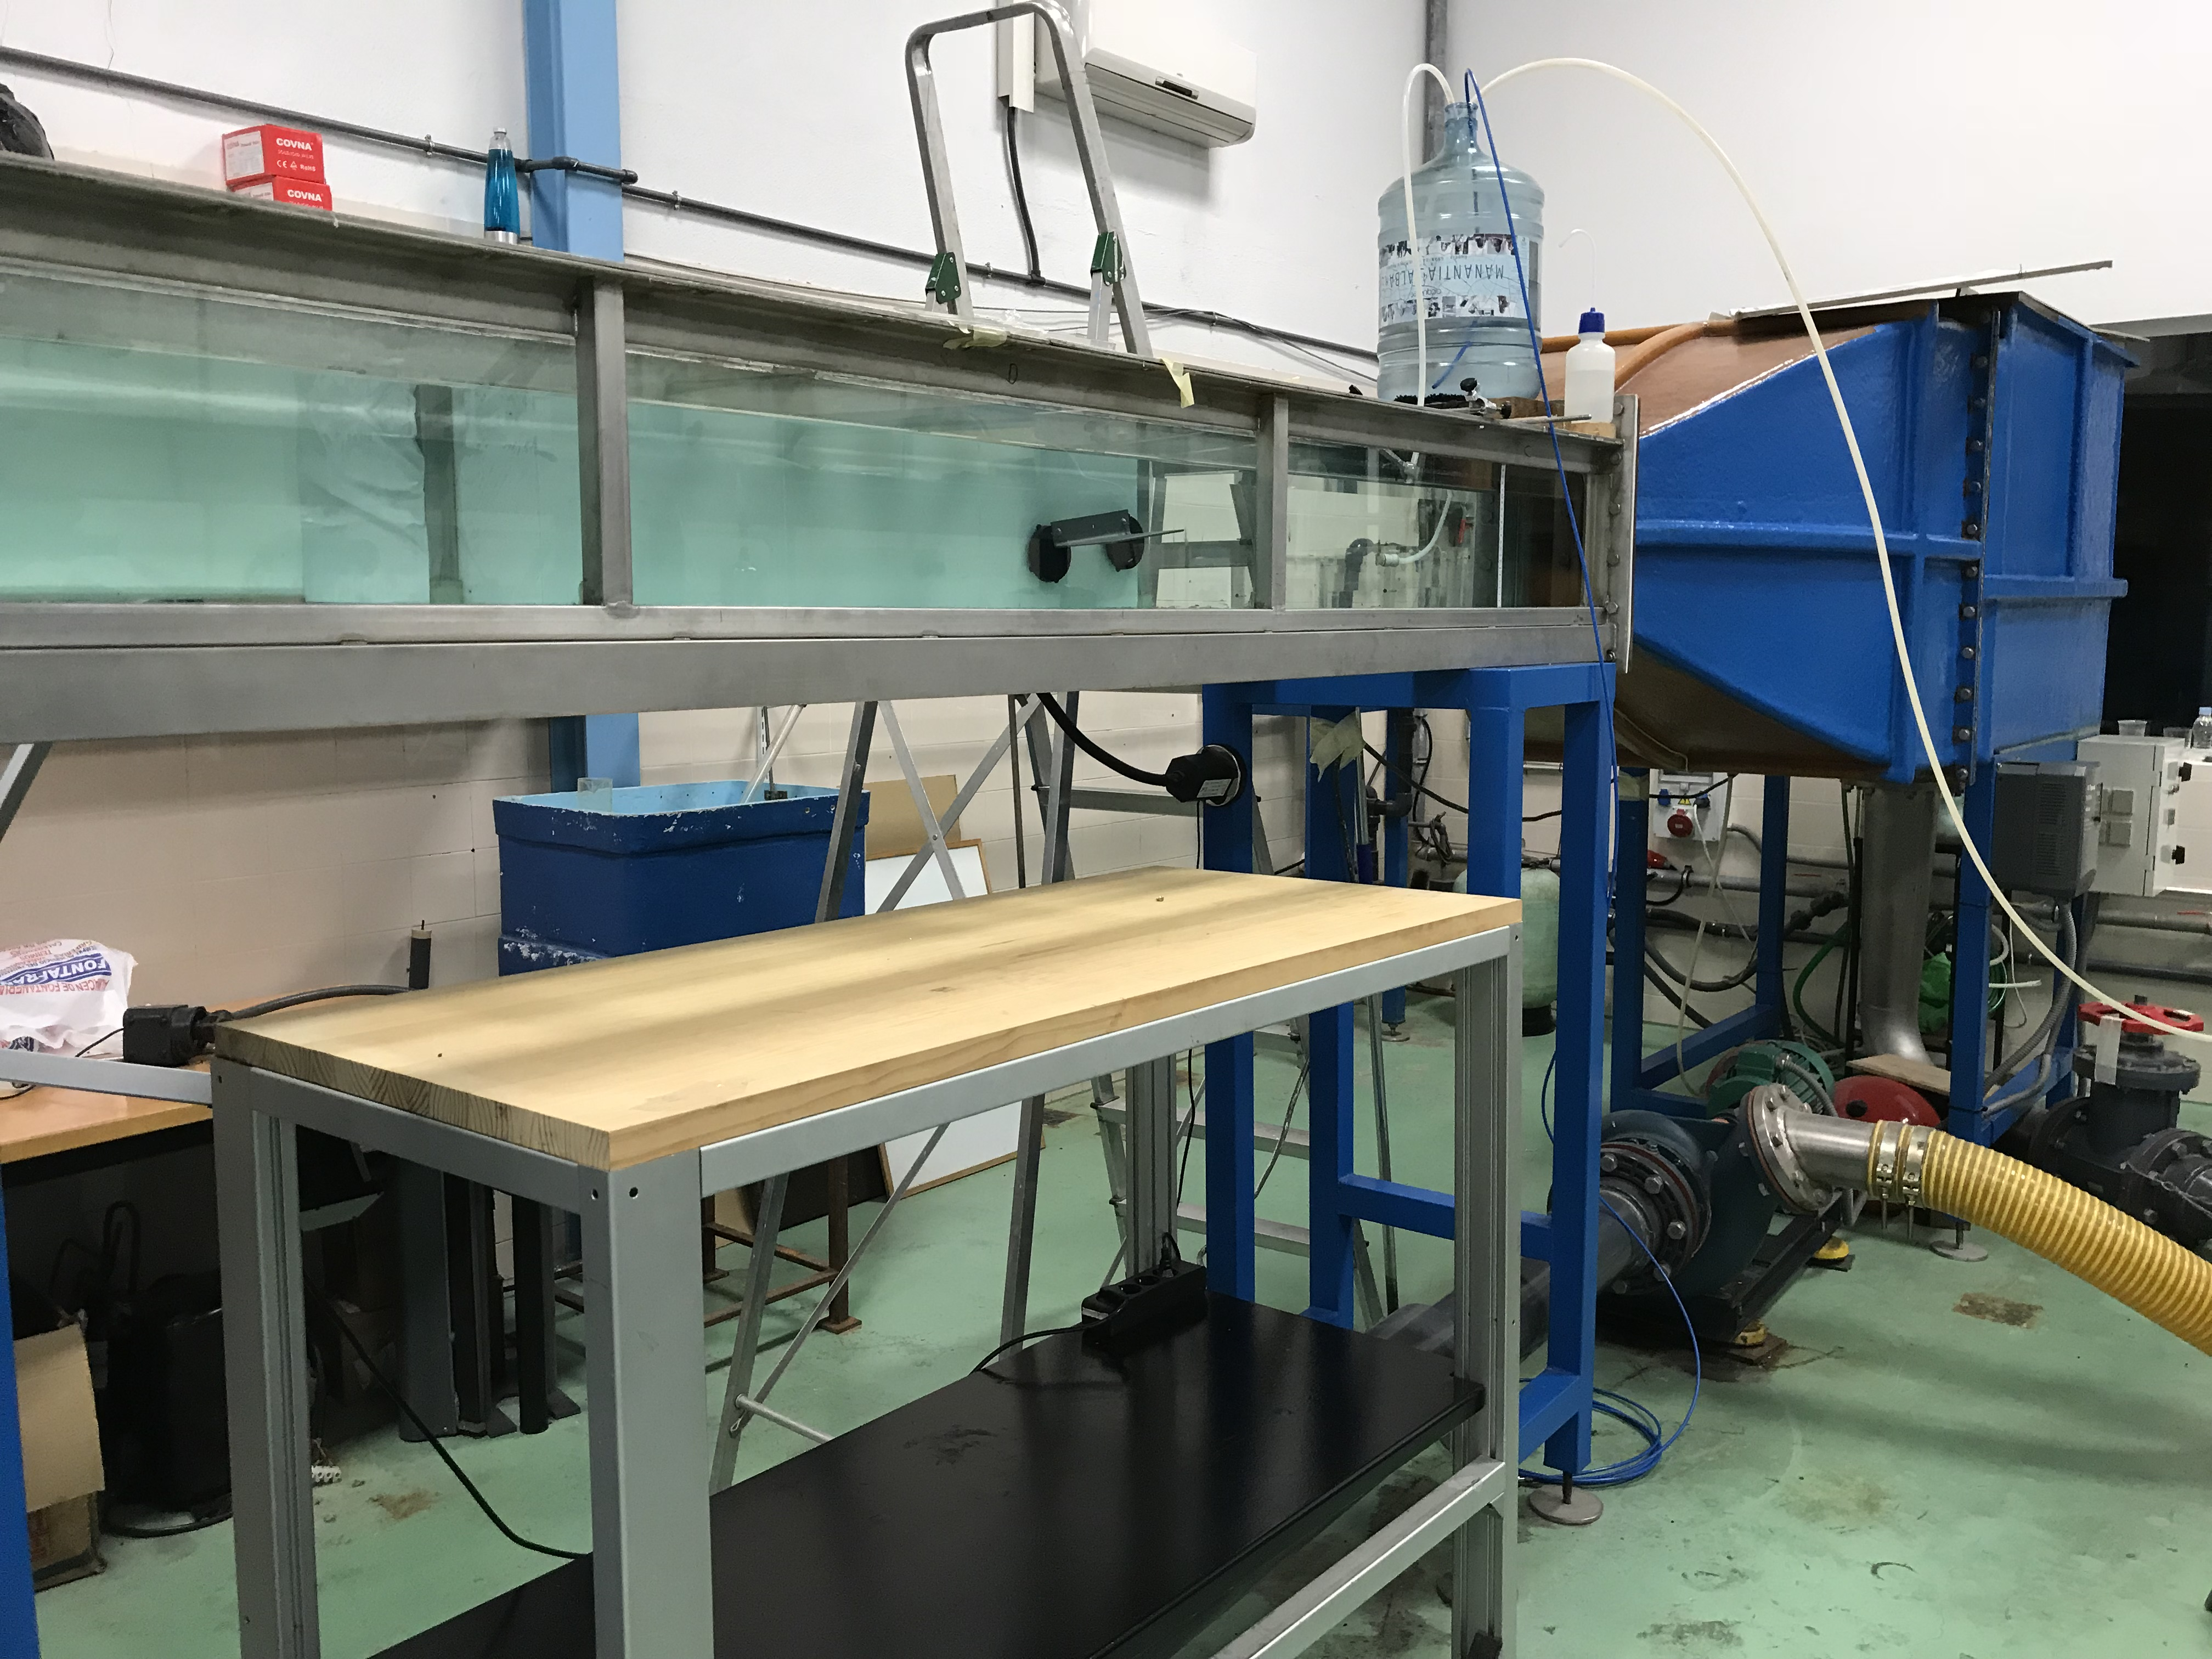
\includegraphics[scale=1]{tunel.jpg}
\caption{Perspectiva del túnel hidrodinámico donde los experimentos han sido realizados.}
\LABFIG{tunel}
\end{figure}

Para el control del caudal que circula a través del túnel hidrodinámico se disponen de dos grados de libertad: la altura total del agua (esto es, la fracción de la sección del túnel que queda mojada) y la velocidad media del agua en la sección. Dado que el túnel se encuentra abierto en su parte superior, se ha comprobado experimentalmente que la velocidad del túnel no puede excederse por encima de $U_{\infty} \sim 0.75\,\mathrm{m/s}$ si se quiere evitar la formación de ondas superficiales. Por lo tanto, se tomará como restricción al diseño que la velocidad de la corriente incidente no puede superar este valor, es decir,

\begin{equation}
U_{\infty} \leq 0.75\,\mathrm{m/s}
\LABEQ{restrVel}
\end{equation}

\subsubsection*{Reguladores de presión}

La formación de burbujas requerirá que se inyecte aire en ciertos puntos de la superficie del ala, el cual debe proceder desde dentro de la misma. Para poder suministrar aire se dispone de una red de presión capaz de suministrar más de 6 bares de presión, lo cual es más que suficiente para el propósito que nos ocupa. Para regular de forma adecuada la presión se dispone de manorreductores cuya precisión es de 1~mbar. 

\subsubsection*{Cámara de alta velocidad}

Se dispone de una cámara Phantom~v710 como la que se muestra en la \FIG{phantom}, capaz de grabar a más de 1~millón de fps. Dado que, según se comentó al inicio de esta sección, serán necesarios en torno a 5000~fps, esta cámara es capaz de acometer dicha tarea sin problema alguno.  Adicionalmente, se disponen de dos objetivos Canon\textsuperscript{\textregistered} diferentes  con zoom 1-4 y 2.5-10, respectivamente. Finalmente, cabe destacar que la distancia focal de la cámara es de aproximadamente 11~cm.


\subsection{Diseño del ala}

Una vez que se consideran los equipos disponibles y las restricciones que pueda imponer cada uno, es momento de pasar a especificar el diseño final del ala. Dado que la sección transversal del ala consiste en un perfil aerodinámico, se ha decidido que el proceso de fabricación sea mediante control numérico, empleando un polímero de ABS (Acrilonitrilo Butadieno Estireno, de sus siglas en inglés) como materia prima. La fabriación por control numérico aúna las ventajas de la impresión~3D y la fabricación tradicional, ya que las paredes de la pieza obtenidas son siempre macizas\footnote{Mediante impresión 3D también es posible emplear un 100\% de entramado, con lo que se obtendrían resultados parecidos con el mismo material; si bien, el empleo de la técnica de impresión 3D con entramados tan elevados suele llevar aparejado un alto coste.} lo que aportará la robustez necesaria para soportar la experimentación del ala en el agua del túnel hidrodinámico.

Para la sección transversal del ala se disponen de dos opciones principales en lo que a perfiles aerodinámicos se refiere: o bien se opta por diseñar un perfil personalizado, o bien se emplea alguno de los perfiles normalizados ya existentes, por ejemplo los de la serie NACA. Se ha elegido para este primer prototipo el conocido perfil simétrico NACA~0012, que posee un espesor máximo relativo a la cuerda $t/c\ = 0.12$. El motivo de empleo de un perfil de estas características se basa principalmente en que el NACA~0012 es uno de los perfiles aerodinámicos más estudiados, lo que unido a la sencillez en su diseño lo hacen idóneo para una primera prueba de concepto. No obstante, el empleo de un perfil con curvatura no supondría una pérdida de generalidad en los resultados obtenidos adelante.

Decidido el perfil aerodinámico que se empleará como sección transversal del ala, tan sólo es necesario definir la cuerda, $c$, y la envergadura, $b$, para tener completamente definida la geometría exterior del ala. Para la cuerda es necesario tener en cuenta los puntos de sujeción que tendrá el ala dentro del túnel hidrodinámico. En principio, podría optarse por disponer de 2 únicos puntos de sujeción (uno a cada lado del ala) que fueran acoplados en torno a una distancia $c/2$ del borde de ataque. Sin embargo, dado que en los experimentos se pretende variar el ángulo de ataque de la corriente inicidente, el diseño de un sistema capaz de variar la inclinación del ala con sólo 2 puntos de sujeción es bastante complejo. Por ello, resulta más sencillo disponer de 4 puntos de sujeción, de forma que se sitúen 2 de ellos cerca del borde de ataque y otros dos cerca del borde de salida, permaneciendo los primeros fijos durante la operación experimental, lo que permite variar la inclinación del ala y con ello el ángulo de ataque $\alpha$ con el que inicide la corriente. El valor que toma la cuerda, de este modo, debe ser tal que permita que el ala se sitúe entre 2 puntos de soporte consecutivos del túnel (véase la \TAB{tunel}), por lo que se ha decidido darle un valor $c = .3\,\mathrm{m}$. En este momento, decida la magnitud de la cuerda,   se está en condiciones de poder calcular el número de Reynolds global en el ala, 

\begin{equation}
Re  = \dfrac{\rho U_{\infty} c}{\mu} \sim \mathcal{O}\left(10^{5}\right) \gg 1. 
\end{equation}

donde se ha tomado un valor orientativo $U_{\infty} \sim 0.5\,\mathrm{m/s}$. Por lo tanto, la magnitud de la cuerda escogida permite sin mayor complicación disponer de las condiciones de $Re \gg 1$ tal y como se pretendía. 

%



%%%%%%%%%%%FIN


\captionsetup[figure]{textformat=period}
\endinput

